\chapter{Antecedentes}

\section{Modelo Estandar}

El Modelo Est\'andar es el formalismo te\'orico-experimental que hasta el d\'{\i}a de hoy  describe con mayor precisi\'on las interacciones entre las part\'{\i}culas elementales y los diferentes tipos de fuerzas que experimentan entre ellas. Los mayores desarrollos teorios y descrubrimientos que dieron forma al Modelo Estandar se dan a partir de la segunda mitad del siglo XX con el desarrollo de la Teoria Cuantica de Campo, fruto del esfuerzo de cientificos de todo el mundo, los cuales a partir de los modelos teoricos y observaciones experimentales construyeron una clasificaci\'on de las particulas en base a sus propiedades fundamentales como lo son la masa, la carga electrica, el espin, entre otras. Dicha clasificacion se muestra en la Figura~\ref{fig:ME}. Las part\'{\i}culas elementales son divididas en dos categor\'{\i}as, los fermiones y los bosones, los fermiones est\'an a su vez divididos en quarks y leptones los cuales tienen un valor fraccional de espin (1/2), adem\'as de que obedecen la estadistica de Fermi-Dirac y el principio de exclusion de Pauli. Los quarks son particulas elementales que constituyen a los hadrones, ya que debido al principio de confinamiento los quarks no pueden co-existir en estado libre.

Cuatro son las fuerzas fundamentales en la naturaleza, la fuerza electromagnetica, la debil, la fuerte y la gravitacional, el modelo estandar incluye las tres primeras, la gravitacional no esta incluida sin embargo su contribucion en la fisica de particulas es despreciable si se compara por ejemplo con la fuerza electromagnetica (una razon de $10^{36}$ a la escala de Giga-electron volts). El modelo estandar esta respaldado por una serie de observacines experimentales, la mas reciente la observaci\'on del boson de Higgs en 2012. Sin embargo aun existen fen\'omenos en la naturaleza que no pueden ser explicados con este formalismo, ejemplo de ellos son: La composicion y naturaleza de la materia y energia oscura.

\begin{figure}
\begin{center}
  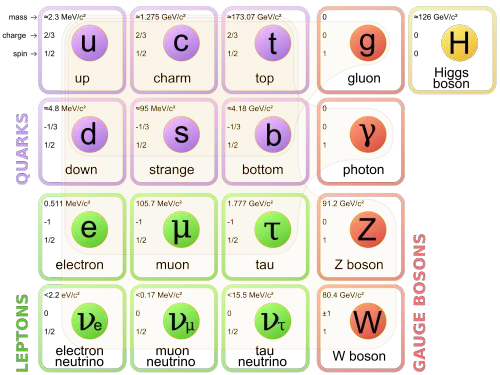
\includegraphics[width=4.0in]{standard-model.png}
  \caption{Clasificaci\'on de las particulas segun El Modelo est\'andar de las part\'iculas elementales}
  \label{fig:ME}
\end{center}
\end{figure}


\section{Materia Oscura}

La materia "oscura" recibe este nombre debido a que no emite radiaci\'on electromagn\'etica, por lo que su existencia se infiere debido a la influencia gravitacional en la materia "visible" o tambien conocida como barionica. A pesar de los diferentes esfuerzos por parte de la comunidad cientifica hasta este momento se desconoce su composicion, por medio de observacones astronomicas se sabe que aproximadamente la materia oscura representa el 30.1\%  de la composici\'on materia-energia del universo, el resto es energia oscura (69.4\%) y materia visible (0.5\%). Recientemente y con el afan de entender la composicion de la materia oscura y su localizacion en el universo la comunidad cientifica ha desarrollado varios experientos, uno de los mas significativos es el Alpha Magnetic Spectrometer (AMS-02) el cual es un detector que busca indicios de materia oscura y antimateria, dicho detector esta instalado en la estacion espacial internaciona (ISS por sus siglas en ingles). En sus observaciones mas recientes se ha observado un flujo de positrones anomalo el cual podria ser explicado como el producto de aniquilacion de particulas de materia oscura~\cite{ams:cern}.  Dicho flujo anomalo puede observarse en la Figura~\ref{fig:AMS_positron} donde tambien se presenta una comparacion con otros experimentos que observan similar comportamiento.  El exceso de flujo observado a partir de los 25 GeV puede tener varias explicaciones cientificas, una de ellas podria ser el resultado de la aniquilacion de particulas de materia oscura. 


\begin{figure}
\begin{center}
  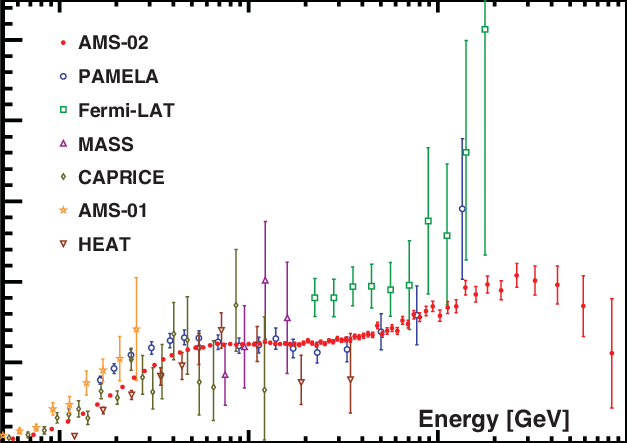
\includegraphics[width=4.0in]{AMS_positronflux.png}
  \caption{Flujo de positrones medido por el experimento AMS-02, comparado con los experimentos PAMELA,Fermi-LAT, MASS, CAPIRCE, AMS-01 y HEAT.}
  \label{fig:AMS_positron}
\end{center}
\end{figure}

Dichas observaciones cosmologicas han motivado a los fisicos de 
altas energias a postular modelos teoricos en los cuales la composicion de la materia oscura se pueda enterder por medio de particulas elementales las cuales podrian estar siendo producidas en los aceleradores de particulas modernos como lo es el Gran Colisionador de Hadrones en Ginebra, Suiza.  Dichos modelos se encuentran clasificados como extensiones al Modelo Estandar y por lo general involucran la existencia de nuevas particulas cuyas fuerzas e interacciones estan descritas por alguna variacion de la Teoria Cuantica de Campo, lo que sugiere puede ser estudiado por el formalismo de la fisica de particulas y estudiado de manera experimental por medio de tecnicas de analisis y analisis estadisticos. 

\chapter{Propuesta}

En este trabajo se propone el estudio de varios modelos teoricos, los cuales se encuentran clasificados como extensiones al modelo estandar y que predicen la creacion de nuevas particulas como producto de la colision de protones altamente energeticos, es decir, los datos que actualmente se producen en el gran colisionador de hadrones del CERN.  En dichos modelos las nuevas particulas pueden ser interpretadas como los constituyentes de la llamada materia oscura.  Usualmente en dichos modelos las nuevas particulas interacciones "debilmente" por lo que su deteccion se daria de forma indirecta, es decir, por su decaimiento a particulas conocidas.  Adicionalmente al estudio de los modelos teoricos se pretende estudiar la parte experimental, la cual consiste en el estudio de la respuesta del detector al paso de las particulas elementales.  La parte experimental es fundamental ya que sin una buena estrategia de seleccion de datos, tecnicas de supresion de ruido y optimizacion de senal seria imposible la observacion de esta nueva fisica. En este proyecto se considera el detector CMS del CERN como el aparato experimental que proporcionara los datos de estudio.  El Experimento CMS es uno de los detectores multi usos del CERN el cual cubre un amplio rango de procesos fisicos que se pueden estudiar, dicho experimento, junto con el experimento ATLAS pudieron observar la particula de Higgs en el 2012.  El experimento consiste de subsistemas los cuales estan disenados para la identifcacion de todas las particulas del modelo estandar, disenado desde suc onstruccion deacuerdo a como cada particula interacciona con la materia, por ejemplo las particulas cargadas son detectadas por detectores de silicio y detectores de gas, ademas de que el signo de la carga es determinado deacuerdo a la defleccion en el campo magnetico solenoide de 4 Teslas.  Las particulas neutras son identificadas por la energia que depositan en los calorimetos.   

En este estuddio se propone el estudio de las senales de nuevas particulas y su paso por el detector por medio de simulacion, de esta manera optimizar la seleccion de los eventos en base a las propiedades de cada modelo, en una segunda fase se pretende estudiar la senal de dichos modelos bajo diferentes escenarios del detector CMS, es decir con el actual detector usado hasta el 2018, durante el llamado periodo 'Run-2'' y el detector que esta disenado para la fase de alta luminosidad, o tambien llamada Phase-2, la cual empezara  a partir del 2025, de esta manera se puede predecir en base a los estudios de simulacion las posibilidades de identificacion de una nueva senal en los proximos anios. 

Dicho estudio es bastante propicio debido a la relevancia de la etapa de alta luminosidad en donde la frecuencia de datos que se acumulara aumentara un factor de 10, es decir la probabilidad de deteccion de nuevas senales sera mucho mayor que la que se tienen con los datos recolectados actualemente, especialmente para el tipo de senales que se desea estudiar. 


\chapter{Justificacion}

Actualmente los modelos teoricos que predicen la formacion de particulas de materia oscura no han sido explorada ampliamente, en gran medida por falta de datos exprimentales que permitan explorar el espacio fase que dichos modelos predicen para esas particulas.  Actualmente con el funcionamiento del gran acelerador de hadrones y sus proyecciones en cuanto a recoleccion de datos en lo proximos anios es la perffecta oportunidad para explotar lo ms posible el estudio de dichos modelos, para en dado caso descubir una nueva senal o en su defecto exlcluir el espacio fase de las particulas predichas. 

\chapter{Hipotesis}
Motivado por recientes observaciones astronomicas, varios modelos teoricos se ha propuesto en el que la materia oscura puede ser descrita por extensiones al modelo estandar. Usualmente se introduce un llamado sector oscuro (dark sector), el cual se comunica con el modelo etandar por medio de un parametro kinematica de mezcla $\epsilon$. Una de las particulas mediadoras del sector oscuro seria el llamado foton oscuro ("dark photon") el cual debido a la interaccion con el modelo estandar decaeria a particulas conocidas, un posible modo de decaimiento es a leptones, uno de los decaimientos posibles es ejemplificado en la Figura~\ref{fig:}.  Dichos decaimientos podrian ser estudiados con los aceleradores de particulas modernos. 


\begin{figure}
\begin{center}
  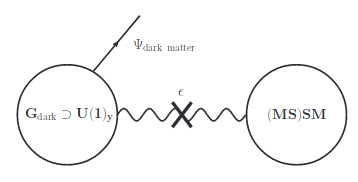
\includegraphics[width=2.8in]{sketch_darksector.png}
  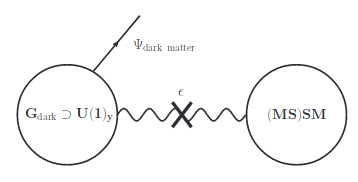
\includegraphics[width=2.8in]{sketch_darksector.png}
  \caption{Ilustracion esquematica de la conexion entre el sector oscuro y el modelo estandar, los cuales estan conectados mediente un termino de mezcla dinamica $\epsilon$}
  \label{fig:AMS_positron}
\end{center}
\end{figure}


\chapter{Objetivo General}

El objetivo principal de este proyecto es el de comprender los diferentes modelos que predicen particulas de materia oscura, estudiar las variaciones de los modelos,  

\chapter{Objetivos Especificos}

\begin{itemize}
    \item Estudio de modelos de fisica mas alla del modelo estandar que predicen la creacion de particulas de materia oscura 
    \item Implementacion de los modelos teoricos en programas de simulacion especializados en fisica de particulas elementales (MADGRAPH, PYTHIA)
    \item Simulacion de los procesos de altas energias por medio del paquete DELPHES 
    \item Analisis de los resultados de simulacion
    \begin{itemize}
        \item Seleccion de eventos 
        \item Eficiencia de la senal y del ruido 
        \item visualizacion de eventos de senal 
        \item Proyecciones de descubrimiento para la fase de alta luminosidad 
    \end{itemize}
\end{itemize}

\chapter{Metodología}

El estudiante seguir una seria de pasos que le permitan estudiar los diferentes modelos de fisica mas alla del modelo estandar, los siguiente pasos pueden resumir 


Produccion de muestras de MonteCarlo: Se espera producir muestras de simulacion de monte carlo para cada proceso de la se\~nal y ruido, el numero de eventos a producir depende del tipo de proceso que se este estudiando y su seccion eficaz, a menor seccion eficaz mayor numero de eventos que se necesitaran producir, las muestras se espera se produzcan usando los recursos computacionales de la Universidad de Sonora. Dicho paso requiere del desarrollo de codigo para la distribucion de las corridas de simulacion en forma paralela usando el cluster ACARUS. Los paquetes de simulacion que se usaran seran MADGRAPH~\cite{Alwall:2007st}, Pythia y Delphes~\cite{deFavereau2014}

Analisis preliminar: El estudiante debe desarrollar diferentes herrammientas de analisis de datos, con el fin de acceder a los datos producidos en la simulacion y extraer las variables de interes, comunmente dichas herramientas de analisis consisten de codigos escritos en lenguaje C++ y python, de esta manera el estudiante dearrollara habilidad en la manipulacion de muestras de datos 

Seleccion de eventos: Despues del acceso de dataos de simulacion y variables de interes se procedera al estudio de la seleccion de eventos, la cual a grandes razgos consiste en seleccionar el conjunto de variables fisicas y valores los cuales puedan optimizar el proceso de senal y reducir lo mas posible la contribucion de ruido 

Analisis estadistico: Despues de la seleccion de eventos se realizara un estudio estadistico en el cual se extraeran el numero de eventos de senal y ruido despues de la seleccion, de ahi se puede interpretar los resultados en base a indicadores estadisticos y concluir la probabibilidad de obsservacion con datos recolectados en los siguientes anos terminao de


\chapter{Resultados Esperados} 

etar en De los estudios de simulaci\'on se espera obtener los siguientes resultados

\begin{itemize}
\item Caracterizacion de los diferentes parametros de los modelos estudiados, asi como las propiedades kinematicas de las diferentes particulas 
\item Las eficiencias de identificacion de particulas 
\item La eficiencia de reconstruccion de particulas 
\item La razon de la senal contra el ruido 
\item La sensitividad de descubrimiento para la etapa de alta luminosidad del experimento CMS
\end{itemize}




